\documentclass[class=book, crop=false]{standalone}
\usepackage[subpreambles=true]{standalone}
\usepackage{import}
\usepackage{amsmath}
\usepackage[margin=1.2in]{geometry}
\usepackage[sorting = none,
            doi = true  %lesedato for url-adresse
            ]{biblatex} %none gir bibliografi i sitert rekkefølge
\addbibresource{reference.bib}
\usepackage{csquotes}

%\usepackage{float}

\begin{document}



%\chapter{Electrical power system}
The reinforcement agent is working within an electrical power system and it is therefore necessary to give an introduction to the electrical grid and relevant quantities describing it. 

\section{Electric circuit theory}
\subsection{Voltage, current and power}
A model of a simple electric circuit is shown in figure \ref{fig:theory:simple_circuit}.

\begin{figure}[ht!]
    \centering
    \subimport{../}{circuits/simple_circuit.tex}
    \caption{Simple electric circuit with voltage source \textit{U}, current \textit{I} and resistance \textit{R}.}
    \label{fig:theory:simple_circuit}
\end{figure}




\textit{U} is the voltage in the circuit and is a measure of the potential energy between charges at each end of the voltage source. volt $V$ is the unit for voltage, which is equivalent to joule per coulomb. The current \textit{I} flowing in the wire is a measure for the amount of charges passing through a cross section of the circuit wire per second. The unit for current is ampere \textit{A} or coulomb per second. The resistance \textit{R} is a measure for how much an electric load resistor, such as a light bulb, resists the flow of electric charges. The unit for resistance is ohm denoted by $\Omega$. The magnitudes of the voltage, current and resistance are governed by Ohm's law

\begin{equation}\label{eq:theory:ohm_simple}
    U = RI
\end{equation}

where  \textit{U} is the voltage, \textit{R} is the resistance and \textit{I} is the current flowing. Another version of this is equation is found by introducing the adittance $Y$ which is defined as the inverse of the resistance $R$, i.e  $Y = 1/R$. The admittance $Y$ is a measure for how a load allows the flow charges in a circuit. The unit for admittance is siemens $S$. By using the admittance $Y$, Ohm's law can be expressed as
\begin{equation}\label{eq:theory:ohm_simple_inverse}
    I = UY
\end{equation}

The power $P$ an electric load consumes can be found easily by multiplying the current \textit{I} and voltage drop \textit{U} over the load
\begin{equation}\label{eq:theory:simple_powerflow}
    P = UI
\end{equation}
The unit for power is watt \textit{W} or joule per second.

\subsection{Kirchoff's laws}
Figure shows a circuit with several branches and resistors 

\begin{figure}[ht!]
    \centering
    \subimport{../}{circuits/simple_circuit_branches.tex}
    \caption{Simple electric circuit with several branches and resistors}
    \label{fig:theory:simple_circuit_branches}
\end{figure}

The current \textit{I} will split when it reaches and intersection, in such a way that the total current flowing into the node equal the total total current flowing out from a node. Referring to figure \ref{fig:theory:simple_circuit_branches} we have that $I = I_1 + I_2$. This conservation of current is called Kirchoff's 1st law or simply kirchhoff current law (KCL). With the introduction of branches in a circuit, there will also be closed loops. In figure \ref{fig:theory:simple_circuit_branches} there are two closed loops $C_{1}$ and $C_{2}$. Kirchoff's 2nd law , aslo known as Kirchoffs's voltage law (KVL), states that the voltage drop over the components in a closed loop $C$ is equal to zero. 

\begin{equation}\label{eq:theory:kirchoffs_2nd_integral}
    \sum_{i}^{N} V_{i} = 0, \;\; V_{i} \in C
\end{equation}
For the two loops $C_1,C_2$ in figure \ref{fig:theory:simple_circuit_branches} we will have 


\begin{equation}
   \begin{aligned}\label{eq:theory:krirchoffs_2nd_ex}
    U + I_{1}R_{1} = 0 
    \\
    -I_{1}R_{1} + I_{2}R_{2} = 0
\end{aligned} 
\end{equation}




\section{Components in the power system}
An electrical power system consists of a set of nodes which can be thought of as the connection points in the system. These nodes are commonly referred to as buses. The connections or branches between the buses are power lines, cables, transformers or other power electronics equipment. The buses and branches defines the topology of the electrical power system. 

\subsection{Types of buses}
There are three types of buses in a power system\cite{opf_intro}.


\begin{itemize}
  \item Slack bus / reference bus
\end{itemize}
Its voltage angle is defined to be 0 and the angles at other buses are relative to the slack bus. There is only one slack bus in an electrical power system.

\begin{itemize}
  \item Load bus
\end{itemize}
A load bus is the most common bus in an electrical grid. The load buses can not control the flow of active and reactive power, as this is predetermined by the demand in the marked. As a result, it is also called PQ bus.

\begin{itemize}
  \item Voltage controlled bus
\end{itemize}
The voltage magnitude and active power are known for the voltage controlled bus, while the voltage angle and reactive power can vary.

\section{Voltage, current and power as complex numbers}
Physical quantities in an alternating current (AC) power system are commonly expressed as a phasor. The voltage $U$ at time \textit{t} in an AC power grid is a sinusoidal signal $U = sin(\omega t)$ where $\omega$ is the angular frequency of the signal. Euler's formula states that a complex number $A$ can be expressed by

\begin{equation}\label{eq:eulers_equation}
    A = e^{j\omega t} = cos(\omega t) + jsin(\omega t)
\end{equation}
where $e$ is the base of the natural logarithm and $j$ is the imaginary unit. The voltage signal could therefore be expressed as $U(t) = Im(A(t))$. The observation making it easy to work with complex numbers in an AC power system is that the angular frequency $\omega$ of the voltages are the same. The frequency of a generator's voltage is directly proportional to the rotational speed of the turbine. If a generator in power system tries to gain speed, it will naturally be slowed down by the other generators in the system, bringing all of the different voltage to the same frequency. Adding two synchronous signals will give a new signal that inherits their frequency. There will be some phase shift to the new signal, but it does not depend on the frequency. As a results, it is possible to treat the sinusoidal signals (such as voltage and current) as a number in the complex plane.  

where \textit{U} is the voltage difference between the two buses which the line is connecting, \textit{Z} is the impedance of the line and \textit{I} is the current flowing in the line. The impedance of a power line is mainly inductive, which results in phase shift between the sinusoidal  current and the voltage difference. 

\section{Two bus system}




\begin{figure}[ht!]
    \center
    \subimport{../}{circuits/two_bus.tex}
    \caption[size = 9]
    {Simple two bus system connected by a line. \textit{P} and \textit{Q} are the active and reactive power flow, \textit{R} and \textit{X} is the resistance and reactance of the line, \textit{U} is the voltage and \textit{I} is the current flowing}    \label{fig:theory:two_bus}
\end{figure}

Figure \ref{fig:theory:two_bus} displays power flow between to buses connected by a transmission line. From the left we have active power $P_{1}$ and reactive power $Q_{1}$ flowing. The power flows through the line and continues out from bus 2 as $P_{2}$ and $Q_{2}$. $U_{1}$ is a complex representation of the voltage at bus 1, $U_{1} = |U_{1}|e^{j\delta}$. Similarly, $U_{2} = |U_{2}|e^{j0} = |U_{2}|$. The relation between voltage and current for the system can be described by Ohm's law.

\begin{equation}\label{eq:chap1_ohm}
    U_{1} - U_{2} = (R + jX)I
\end{equation}
$R$ is the resistance and $X$ is the reactance of the line, $U_{1}$ and $U_{2}$ are the voltages at bus 1 and 2, and \textit{I} is the current flowing in the line. The impedance \textit{Z} of the line is also a complex number that can be expressed as $Z = |Z|e^{j\epsilon}$ where $tan (\epsilon) = X/R$. The current \textit{I} is commonly defined to be lagging, so that $I = |I|e^{-j\varphi}$. By this definition, $\varphi$ is a positive real number when the current is lagging the voltage. In figure \ref{fig:two_bus_phasor}, the current, voltages and impedance are drawn as phasors in the complex plane for a line with zero resistance (R=0).


\begin{figure}[ht!]
    \center
    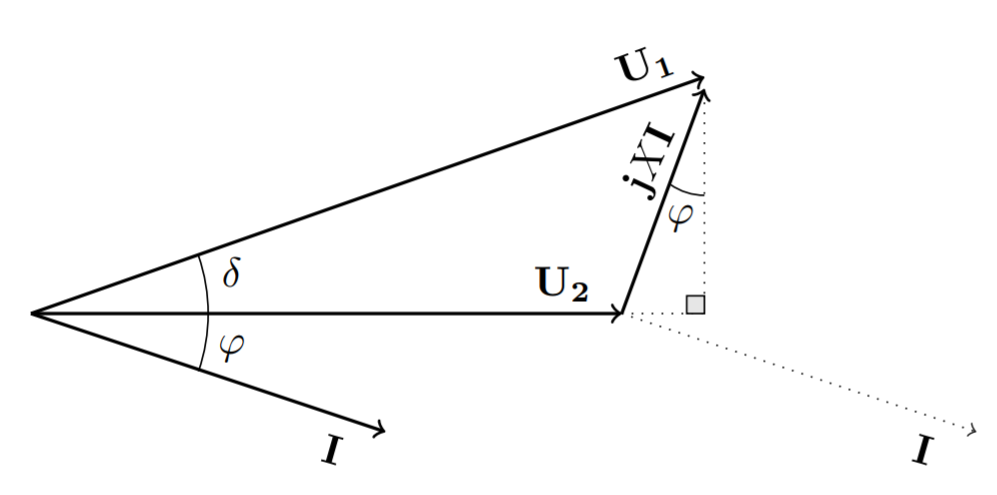
\includegraphics[width=10cm]{figures/two_bus_phasor.PNG}
    \caption[size = 9]{Phasors of current and voltages in a two-port network connected by line with 0 resistance (R=0)}
	\label{fig:two_bus_phasor}
\end{figure}

The apparent power $S$ flowing in a line is defined to be
\begin{equation}\label{eq:apparent_power}
    S  = UI^{*} = P + jQ
\end{equation}

Where \textit{U} is the voltage, $I^{*}$ is the complex conjugate of the current, \textit{P} is the active power and \textit{Q} is the reactive power. The conjugation of the current is a convenience to make the reactive power \textit{Q} a positive number when the current is lagging the voltage. Using using \eqref{eq:chap1_ohm}, the current \textit{I} in the line can be expressed as

\begin{equation}\label{eq:two_port_current}
    I  = \frac{U_{1} - U_{2}}{Z}
    = \frac{|U_{1}|e^{j\delta} - |U_{2}|}{|Z|e^{j\epsilon}}
    = \frac{|U_{1}|e^{j(\delta- \epsilon)} - |U_{2}|e^{-j\epsilon}}{|Z|}
\end{equation}
where $|U_{1}|$ and $|U_{2}|$ are the voltage magnitudes at bus 1 and 2, \textit{I} is the current flowing in the line and \textit{|Z|} is the impedance magnitude for the line. Using the definition of power flow in \eqref{eq:apparent_power} on bus 1 gives that the active power $P_{1}$ is given by

\begin{equation}\label{eq:two_port_active_power}
P_{1} = \frac{|U_{1}|^2}{|Z|}cos(\epsilon) - \frac{|U_{1}||U_{2}|}{|Z|}cos(\epsilon - \delta)
\end{equation}
To make it easier to investigate a situation with active losses in the line (R = 0), it is convenient to introduce a loss angle $\alpha = tan(R/X)$. By the sum of angles in a triangle, we have the relation $\alpha + \epsilon = \pi/2$. By using the loss angle $\alpha$, the active power at bus 1 $P_{1}$ can be expressed as

\begin{equation}\label{eq:two_port_active_power_good}
P_{1} = \frac{|U_{1}|^2}{|Z|}sin(\alpha) + \frac{|U_{1}||U_{2}|}{|Z|}sin(\delta -\alpha)
\end{equation}
A line without resistive losses can now be examined simply by setting $\alpha = 0$. The resulting active power flow $P_{1}$ reduces to

\begin{equation}\label{eq:two_port_active_power_lossless}
P_{1} =  \frac{|U_{1}||U_{2}|}{|Z|}sin(\delta)
\end{equation}
where $|U_{1}|$ and $|U_{2}|$ are the voltage magnitudes at bus 1 and 2, $|Z|$ is the impedance magnitude of the line and $\delta$ is the phase angle at bus 1 with respect to bus 2. The takeaway from this analysis is that the direction of the active power flow is determined by the phase angle $\delta$ of the voltages between the buses. In a two bus system, the bus with the leading voltage is supplying active power, while the lagging voltage is receiving. Another thing to note is that for an AC power system the voltage magnitude between the buses may differ in size, and active power can still flow in both directions. This would not be possible in DC power system. Figure \ref{fig:theory:active_power_flow} shows the relation between a loss free power line and a sample line in pandapower. We see that the active power $P$ for a line with resistive losses is also mainly controlled by the voltage angle $\delta$.


\begin{figure}[ht!]
    \center
    \subimport{../}{circuits/plot_active_power_flow.tex}
    \caption[size = 9]{Active power flow \textit{P} between two buses as a function of voltage angle with no losses ($\alpha=0$) a and typical loss angle $\alpha$ of 0.13} \label{fig:theory:active_power_flow}
\end{figure}

A similar argument will give that the reactive power flow $Q_{1}$ at bus 1 for a line without resistive losses is given by 

\begin{equation}\label{eq:two_port_reactive_power_lossless}
Q_{1} =  \frac{|U_{1}|}{|Z|}(|U_{1}| - |U_{2}|)
\end{equation}
where $|U_{1}|$ and $|U_{2}|$ are the voltage magnitudes at bus 1 and 2 respectively and $|Z|$ is the impedance magnitude of the line. The voltage angle $\delta$ is assumed to be small so that $cos(\delta) \approx 1$. Equation \eqref{eq:two_port_reactive_power_lossless} shows that the direction of the reactive power is determined by the difference of the voltage magnitudes. In other words, the bus with the highest voltage magnitude is supplying reactive power in a two bus system.

\section{Power flow in a grid}
Figure \ref{fig:power_flow_network} is an electrical model of bus \textit{k} in a power system that is connected to \textit{n} buses. $I_{k}$ is the net injected current to the grid from bus \textit{k}\cite{opf_intro}. It is common to work with the admittance $Y$ of a line, which is defined as the inverse of the impedance $Y = 1/Z$. By doing this, the current in a branch is easily found by multiplying the voltage difference and the admittance. The current flowing from bus \textit{k} to bus \textit{j} is $I_{j} = (U_{k} - U_{j})Y_{kj}$. The current flowing out of bus \textit{k} must equal the injected current $I_{k}$. This gives

\begin{equation}\label{eq:powerflow_currentsum}
I_{k} =  U_{k}Y_{k0}
+ \sum_{j=1,j\neq k}^{n}(U_{k} - U_{j})Y_{kj}
\end{equation}


\begin{figure}[ht]
    \center
    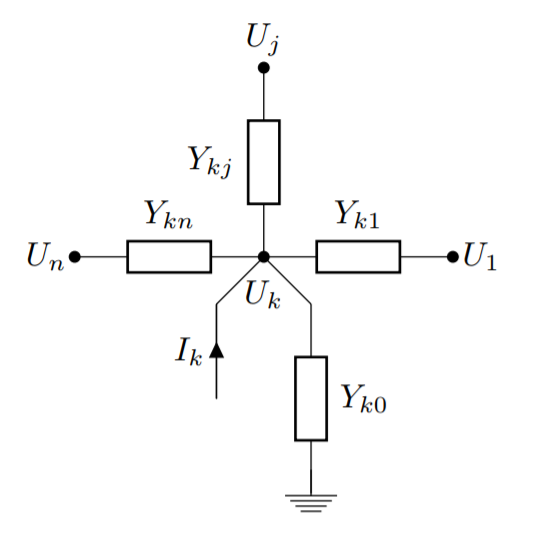
\includegraphics[width=8cm]{figures/power_flow_network.PNG}
    \caption[size = 9]{Electrical model of a bus connected to n buses}
	\label{fig:power_flow_network}
\end{figure}

This is a linear system of equation that can be expressed compactly as a matrix equation with the bus voltages ordered in a vector $U_{bus}$

\begin{equation}\label{eq:powerflow_busmatrix}
I_{bus} = Y_{bus}U_{bus}
\end{equation}
where $I_{bus}$ are n-dimensional vectors whose j-th component is the current flowing from \textit{k} to bus \textit{j}.


\section{Electric model of a power line}
A common way to model a transmission line is by using a $\pi$-equivalent circuit, as shown in figure \ref{fig:theory:PI_model}

\begin{figure}[ht!]
    \subimport{../}{circuits/pi_model.tex}
    \caption{$\pi$-equivalant model for a transmission line.}
    \label{fig:theory:PI_model}
\end{figure}



The transmission line is modelled by a resistance and inductance in series. In addition, there are two shunt capacitors connected in parallel at each end of the line. The capacitors are there because the flow of charges will give an associated capacitance that is proportional with the line length. The $\pi$-model splits the admittance $Y$ of the capacitor into two and puts one part on each end of the line. It is this model pandapower uses to solve a given transmission system. 



\end{document}
